 \section{Experimental Results}
In this section, we evaluate our proposed approach and present the results of applying our method to various images. Our experiments were conducted on several images from \cite{draa2014artificial} and additional images (color, grayscale, and text) sourced from the Internet. Specifically, we experimented with a total of 18 images.

\subsection{Experimental Setup and Environment}
To evaluate the efficacy of our approach, we implemented a prototype in Python using the DEAP evolutionary computation framework\footnote{\url{https://deap.readthedocs.io/en/master/}}. For the fuzzy logic component, we utilized the scikit-fuzzy toolbox\footnote{\url{https://pythonhosted.org/scikit-fuzzy/}}.

All variants of our algorithms were executed on a system with an Intel(R) Core(TM) i$3$ CPU M$370$ @ $2.40$GHz processor, $6$GB RAM, running Ubuntu $18.04$, and Python version $3.6.8$.
% will be available after acceptance
% Our experiment code can be found in this link, \href{https://dicta2024.dictaconference.org/}{redacted for review version}.

\subsection{Results}
\label{subsection:exp_result_result}

Here, we visually present outputs for a limited number of images due to our page limitation. Figures \ref{fig:07_output_image_hc}, \ref{fig:jetplane_output_image_hc}, \ref{fig:07_output_image_ga}, \ref{fig:house_output_image_ga} show output images generated by our technique against the reference input images.
As an outcome of our technique, the enhanced images are more clear and natural (Figures~\ref{fig:07_output_image_hc}, \ref{fig:07_output_image_ga}, \ref{fig:house_output_image_ga}), the edges are sharper (Figures \ref{fig:jetplane_output_image_hc},
\ref{fig:house_output_image_ga}), the histogram is expanded, and the contrast between black and white portion is increased. On the contrary, some black portions (Figures \ref{fig:jetplane_output_image_hc}, \ref{fig:07_output_image_ga}) are unnecessarily darkened. 

\subsection{Survey}
\label{subsection:exp_result_survey}
\subsubsection{Variant Selection to Select Survey Images}
First, we have grouped the variants according to used metaheuristic algorithms, namely Hill Climbing and Genetic algorithm. Then according to the method described in Subsection \ref{subsection:experiment_process}, we have ranked the variants among two groups. Based on this the selected variants from the two groups are as follows:
\begin{enumerate}
    \item (Method $1$) Hill Climbing with simple neighborhood generation (Subsection \ref{subsubsec:simple_neighbour_generation})
    \item (Method $2$) Genetic Algorithm with (P, P) strategy (Subsection \ref{subsection:method_ga_join})
\end{enumerate}

\subsubsection{Survey Preparation}
We have prepared an anonymous survey %\footnote{\url{https://forms.gle/9wuLKMYBShjyAaK59}} 
to get a quantitative opinion on our enhanced images. In the survey, we have placed $36$ enhanced images (produced by our technique) side-by-side with their original image. The first $18$ images are from Hill Climbing with neighborhood generation with split mutation (see Section \ref{subsubsection:method_hc_traptri_split}), and the second $18$ images are the same but from the Genetic Algorithm with (P, P) strategy (see Section \ref{subsection:method_ga_join}). The survey participant needs to mark the enhanced image on a scale of $1-9$. As the reference, the mark of the original image was $5$; therefore, a mark of $>5$ by the reviewer would mean an enhanced image, while $<5$ will mean image degradation. A mark of $5$ would mean the processed image is the same as the original visually (a subjective judgment). The prepared survey form can be found at the following link: \href{https://dicta2024.dictaconference.org}{redacted for review version}%\url{https://forms.gle/9wuLKMYBShjyAaK59}.
%\href{https://forms.gle/9wuLKMYBShjyAaK59}{here}.

\subsubsection{Survey Response \& Observations}
We have received a total of $67$ responses. From the responses, we have filtered responses with suspicious patterns like all equal marks or very high or very low marks. This filtering caused two responses to be filtered. From the remaining $65$ responses, it seems method $2$, achieving a mean score of $5.45$, is better than method $1$, achieving a mean score $4.77$. 
Moreover, achieving a mean score of greater that $5$ indicates that the method $2$ improves the original image.

\begin{figure}[!htb]
\begin{subfigure}{0.5\textwidth}%
  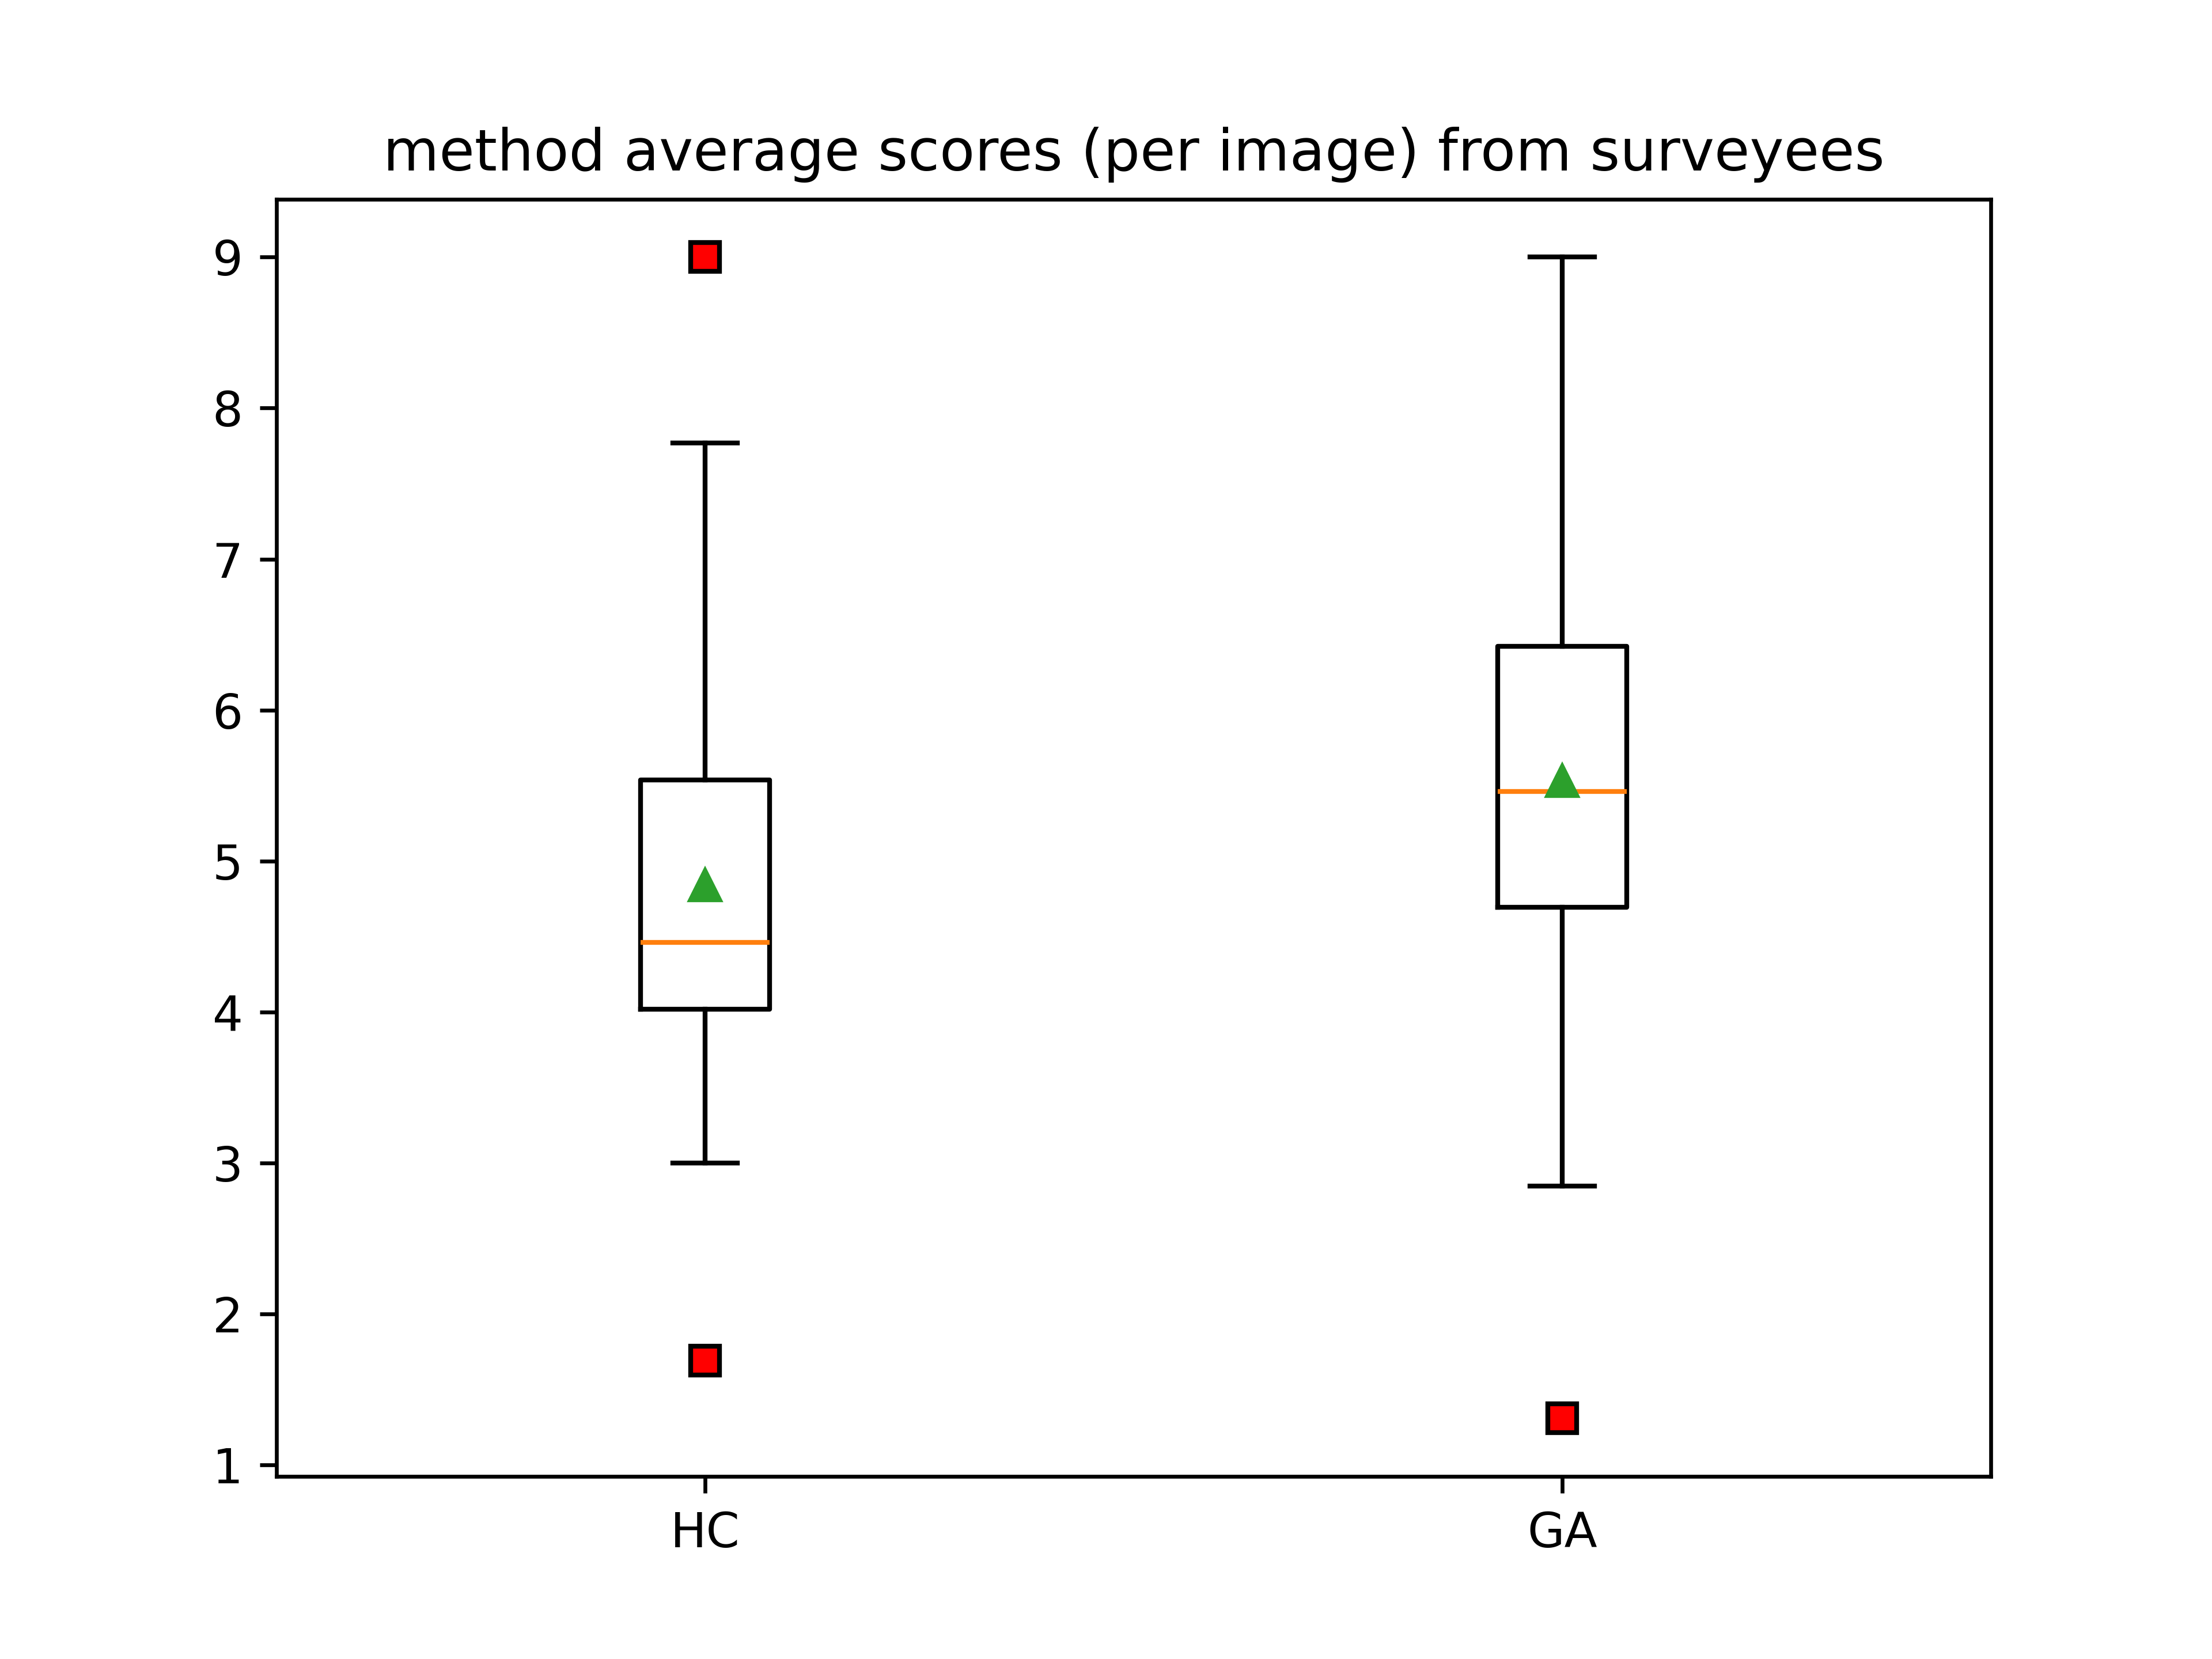
\includegraphics[width=\linewidth]{surveyee_score_box_plot.png}
  \caption{}
  \label{fig:survey_result_boxplot}
\end{subfigure}
\begin{subfigure}{0.5\textwidth}%
  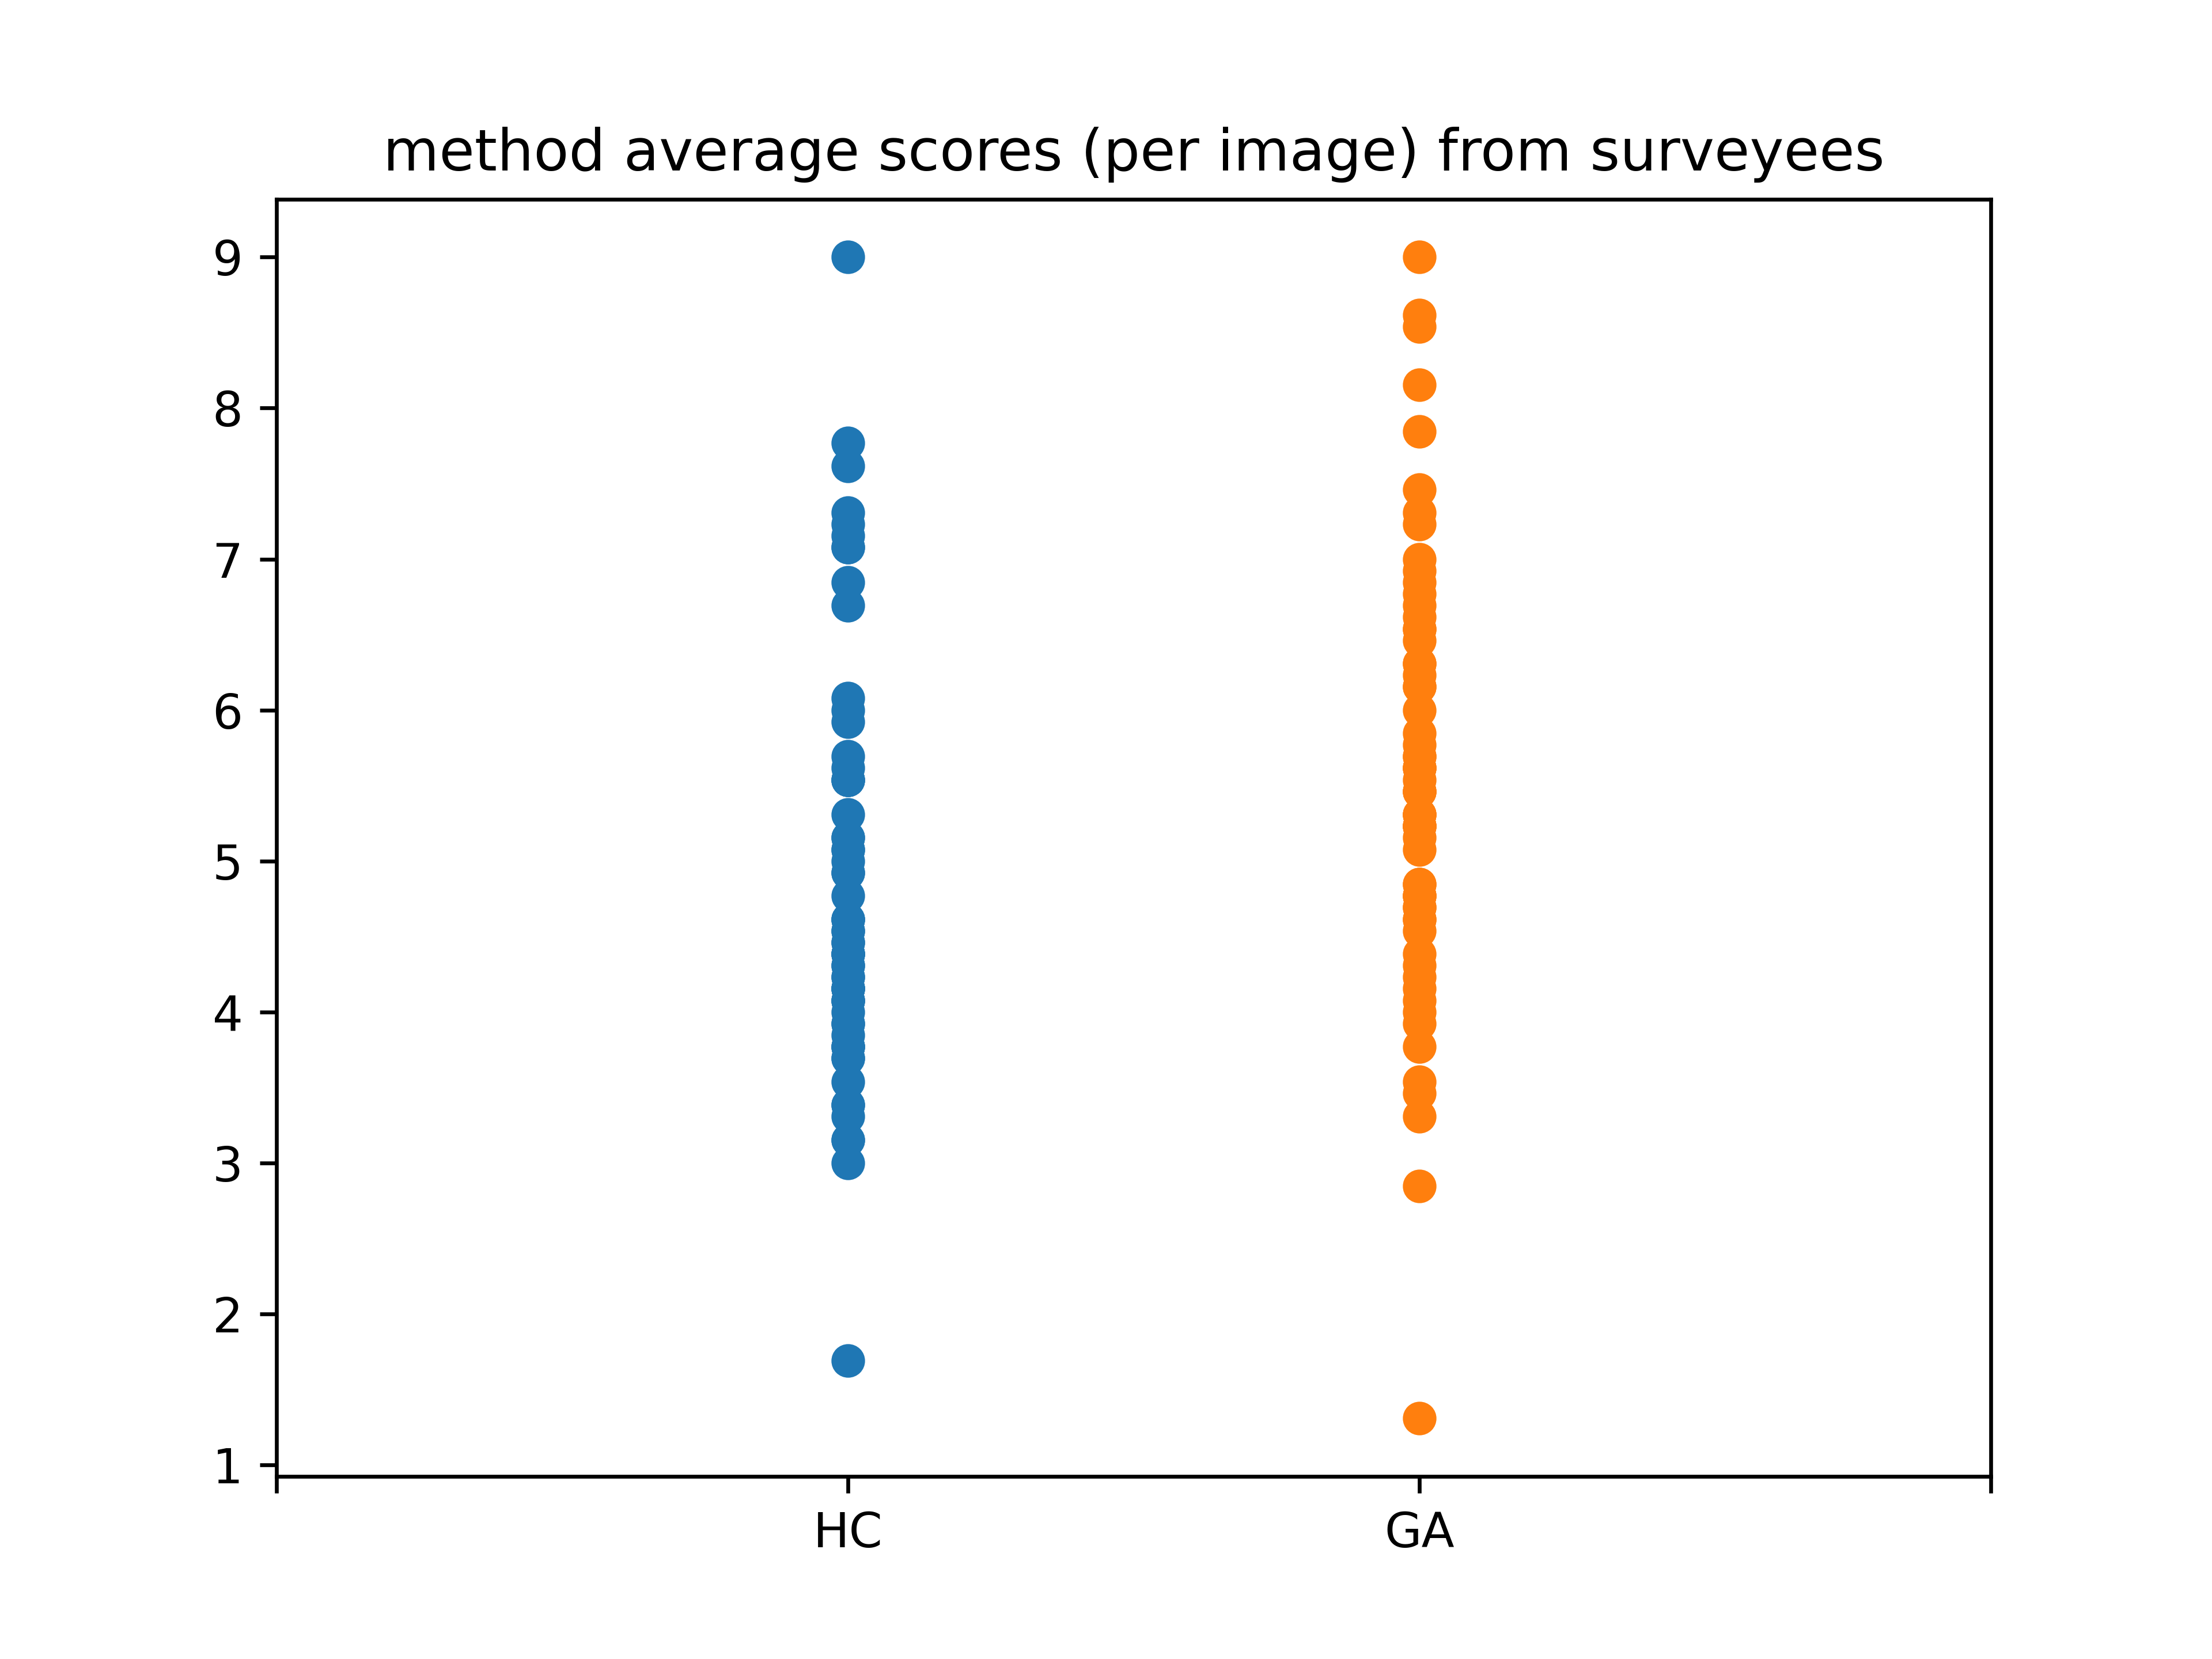
\includegraphics[width=\linewidth]{surveyee_score_scatter_plot.png}
  \caption{}
  \label{fig:survey_result_scatterplot}
\end{subfigure}
  \caption{Box plot of achieved score from survey participants of two methods. Method $1$ represents Hill Climbing with neighborhood generation with split mutation (\ref{subsubsection:method_hc_traptri_split}) and method $2$ represents Genetic Algorithm with (P, P) strategy (see Section \ref{subsection:method_ga_join}) }
  \label{fig:survey_result}
\end{figure}

From Figure \ref{fig:survey_result}, we can see the mean scores of all enhanced images given by each surveyee. 
Each data point in Figure \ref{fig:survey_result}(b) indicates the mean of scores given by one participant. Figure \ref{fig:survey_result}(a) shows the mean (triangle inside each box, green in color picture), and median (horizontal line inside each box, orange in color picture) of the responses. The red points are outliers according to the $1.5 \times$IQR rule \cite{rousseeuw2011robust}.

From Figure \ref{fig:survey_result}(a), method $2$ shows a better mean score than method $1$'s mean score (mean over participants). From Figure \ref{fig:survey_result}(b), we can see that method $1$ has a higher chance of degrading the image (dense below score $5$), although method $2$ has achieved the image with the lowest score according to one participant.

\begin{figure*}
  % one image
  \begin{subfigure}[b]{0.33\textwidth}%
    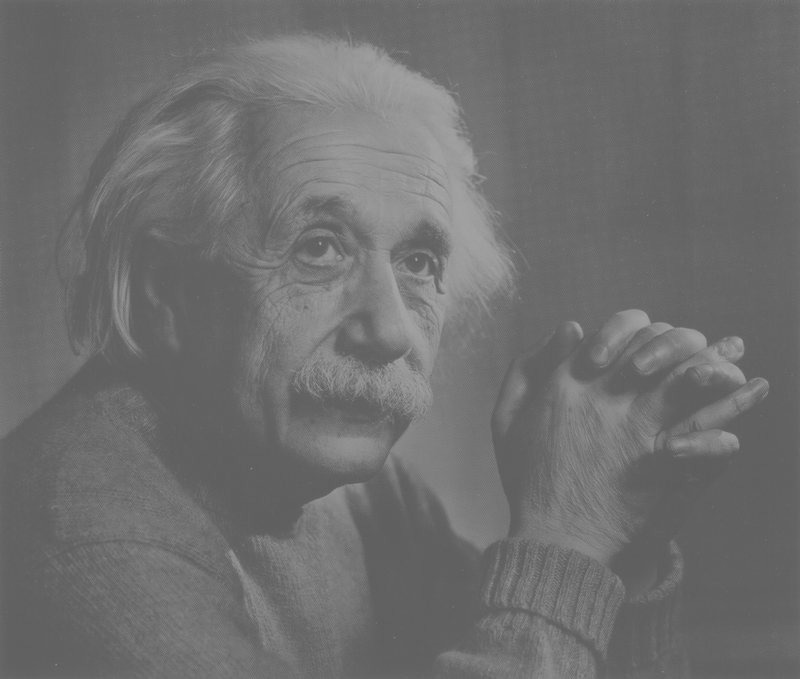
\includegraphics[width=\linewidth]{figures/original/07.jpg}
    \subcaption[]{}{}
    \label{fig:07_image_original}
  \end{subfigure}
  \begin{subfigure}[b]{0.33\textwidth}%
    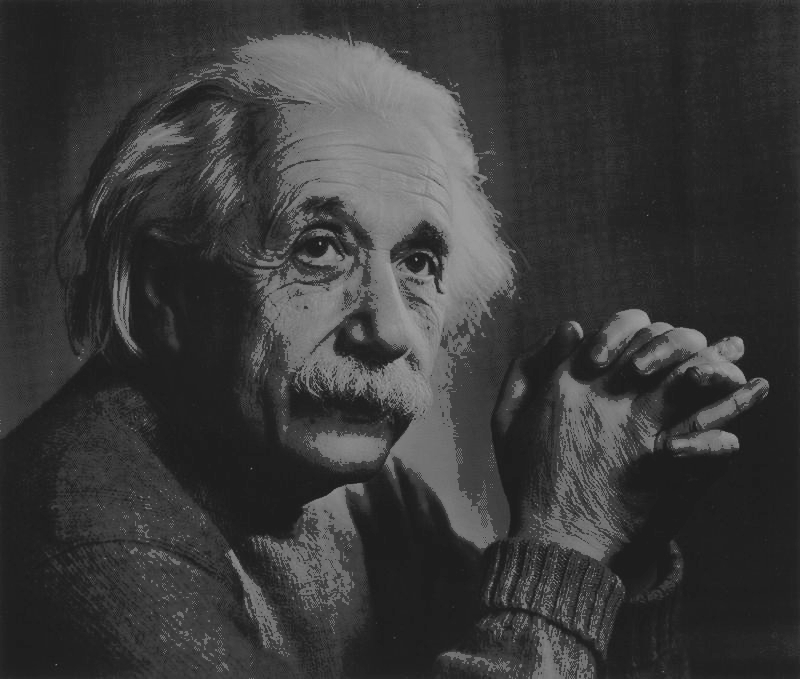
\includegraphics[width=\linewidth]{figures/hc_trap_split/07_output.jpg}
    \subcaption[]{}{}
    \label{fig:07_output_image_hc}
  \end{subfigure}
  \begin{subfigure}[b]{0.33\textwidth}%
    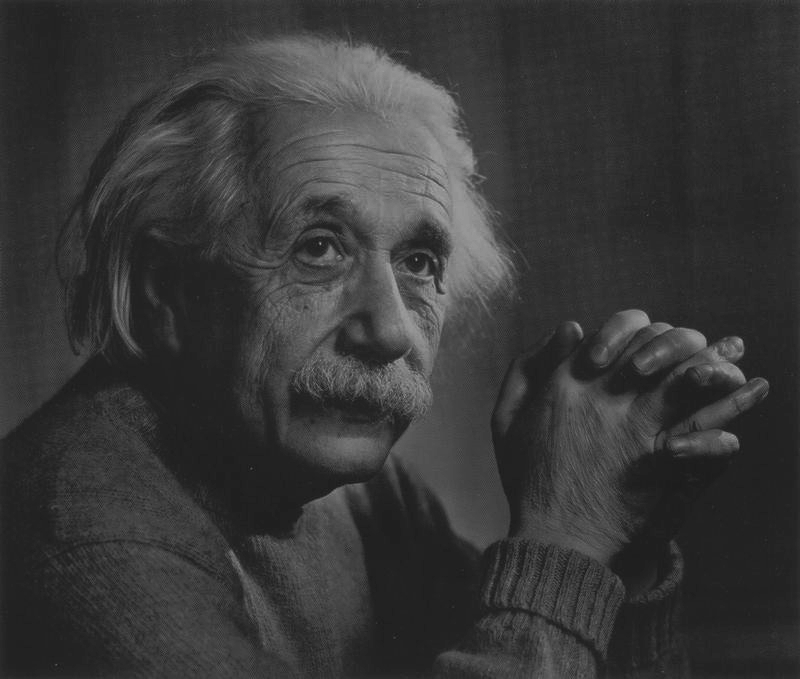
\includegraphics[width=\linewidth]{figures/ga_elitist/07_output.jpg}
    \subcaption[]{}{}
    \label{fig:07_output_image_ga}
  \end{subfigure}
  \vspace{-15pt}
  \caption{enhanced image generated by (b) simple HC (c) GA and (a) is original image}
  \label{fig:07_result}

  % one image
  \begin{subfigure}[b]{0.33\textwidth}
    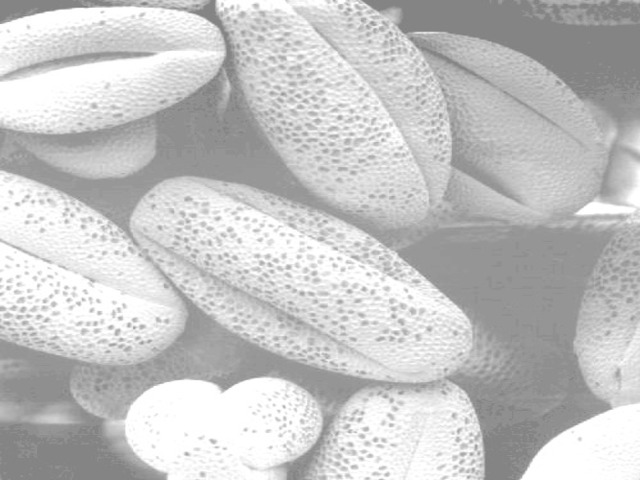
\includegraphics[width=\linewidth]{figures/original/08.jpg}
    \subcaption[]{}{}
    \label{fig:08_image_original}
  \end{subfigure}
  \begin{subfigure}[b]{0.33\textwidth}%
    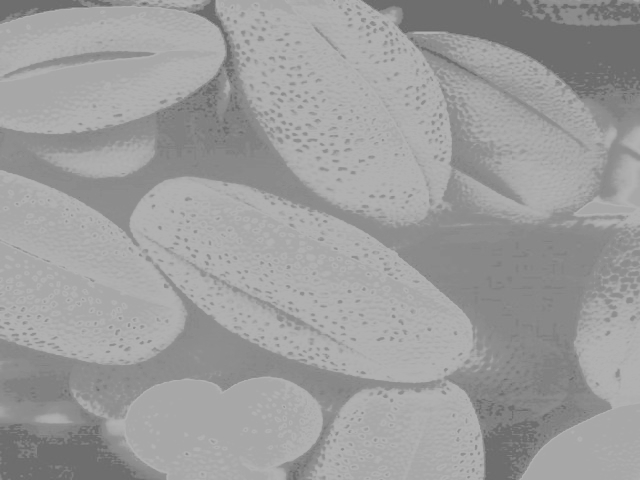
\includegraphics[width=\linewidth]{figures/hc_trap_split/08_output.jpg}
    \subcaption[]{}{}
    \label{fig:08_output_image_hc}
  \end{subfigure}
  \begin{subfigure}[b]{0.33\textwidth}%
    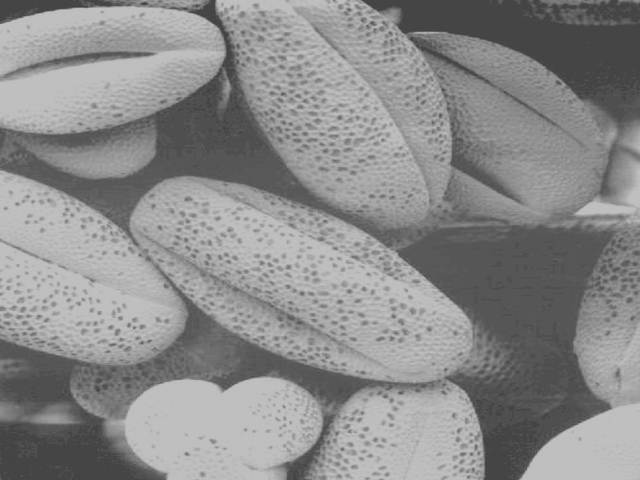
\includegraphics[width=\linewidth]{figures/ga_elitist/08_output.jpg}
    \subcaption[]{}{}
    \label{fig:08_output_image_ga}
  \end{subfigure}
  \vspace{-15pt}
  \caption{enhanced image generated by (b) simple HC (c) GA and (a) is original image}
  
  \label{fig:08_result}

  % one image
  \begin{subfigure}[b]{0.33\textwidth}
    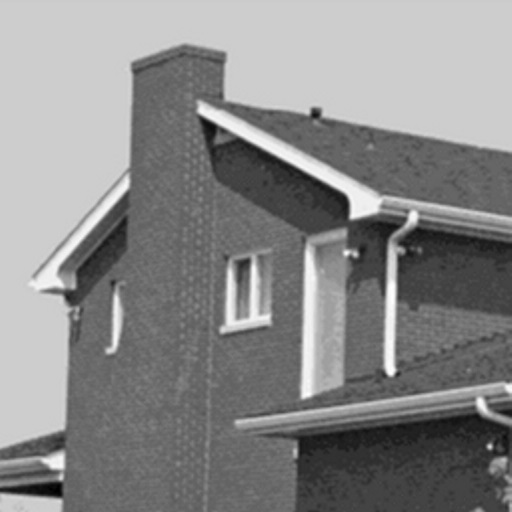
\includegraphics[width=\linewidth]{figures/original/house.jpg}
    \subcaption[]{}{}
    \label{fig:house_image_original}
  \end{subfigure}
  \begin{subfigure}[b]{0.33\textwidth}%
    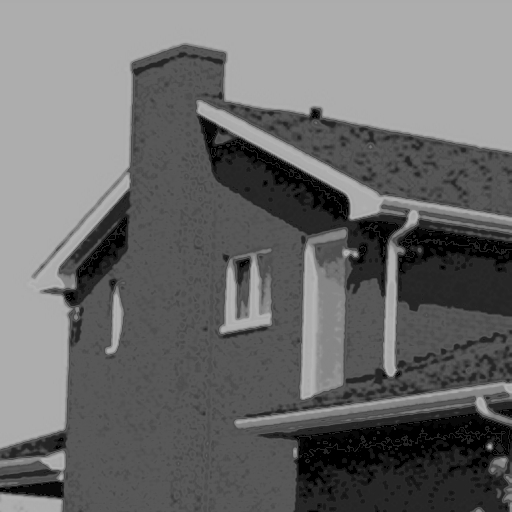
\includegraphics[width=\linewidth]{figures/hc_trap_split/house_output.jpg}
    \subcaption[]{}{}
    \label{fig:house_output_image_hc}
  \end{subfigure}
  \begin{subfigure}[b]{0.33\textwidth}%
    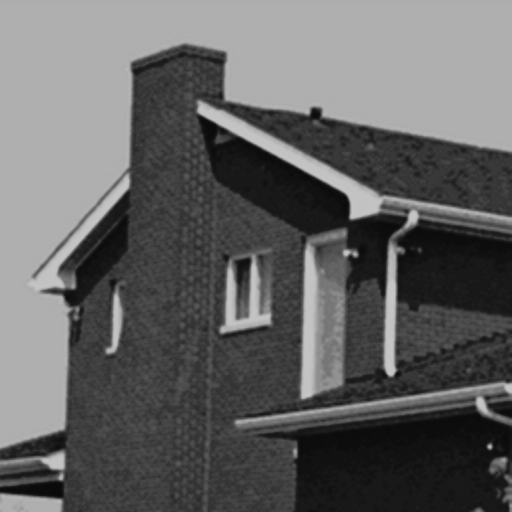
\includegraphics[width=\linewidth]{figures/ga_elitist/house_output.jpg}
    \subcaption[]{}{}
    \label{fig:house_output_image_ga}
  \end{subfigure}
  \vspace{-15pt}
  \caption{enhanced image generated by (b) simple HC (c) GA and (a) is original image}
  \label{fig:house_result}

  % one image
  \begin{subfigure}[b]{0.33\textwidth}
    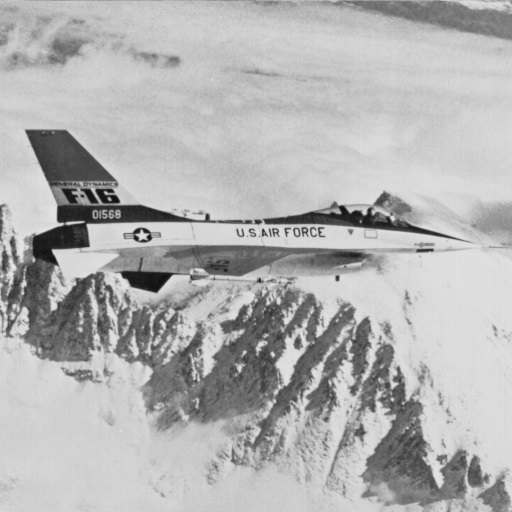
\includegraphics[width=\linewidth]{figures/original/jetplane.jpg}
    \subcaption[]{}{}
    \label{fig:jetplane_image_original}
  \end{subfigure}
  \begin{subfigure}[b]{0.33\textwidth}%
    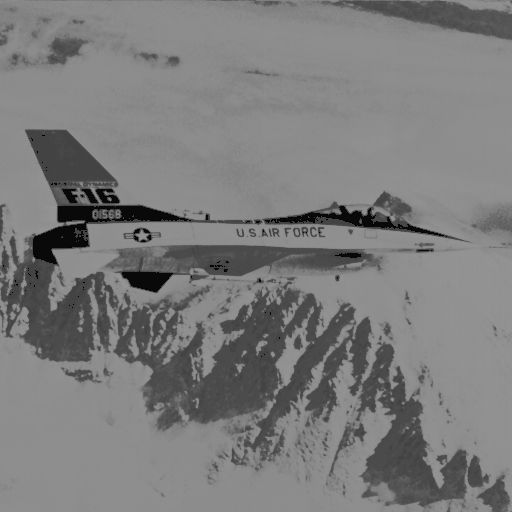
\includegraphics[width=\linewidth]{figures/hc_trap_split/jetplane_output.jpg}
    \subcaption[]{}{}
    \label{fig:jetplane_output_image_hc}
  \end{subfigure}
  \begin{subfigure}[b]{0.33\textwidth}%
    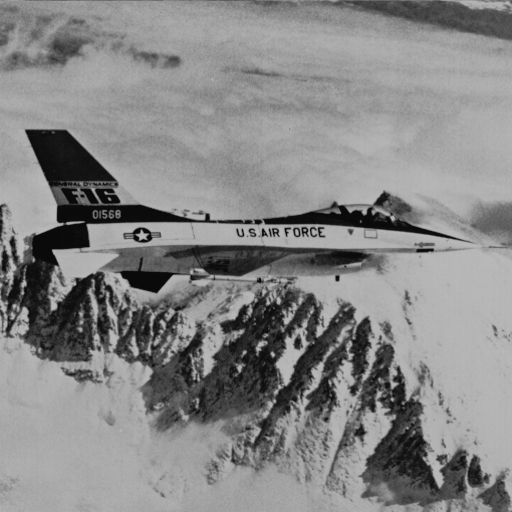
\includegraphics[width=\linewidth]{figures/ga_elitist/jetplane_output.jpg}
    \subcaption[]{}{}
    \label{fig:jetplane_output_image_ga}
  \end{subfigure}
  \vspace{-15pt}
  \caption{enhanced image generated by (b) simple HC (c) GA and (a) is original image}
  \label{fig:jetplane_result}
\end{figure*}

% next page
\begin{figure*}
  % one image
  \begin{subfigure}[b]{0.33\textwidth}
    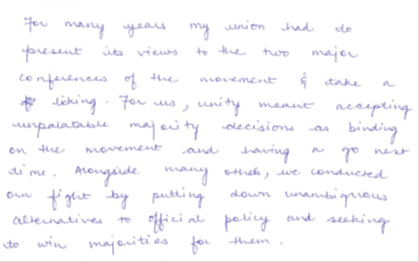
\includegraphics[width=\linewidth]{figures/original/11.png}
    \subcaption[]{}{}
    \label{fig:11_image_original}
  \end{subfigure}
  \begin{subfigure}[b]{0.33\textwidth}%
    
\includegraphics[width=\linewidth]{figures/hc_trap_split/11_output.jpg}
    \subcaption[]{}{}
    \label{fig:11_output_image_hc}
  \end{subfigure}
  \begin{subfigure}[b]{0.33\textwidth}%
    
\includegraphics[width=\linewidth]{figures/ga_elitist/11_output.jpg}
    \subcaption[]{}{}
    \label{fig:11_output_image_ga}
  \end{subfigure}
  \caption{enhanced image generated by (b) simple HC (c) GA and (a) is original image}
  \label{fig:11_result}

  % one image
  \begin{subfigure}[b]{0.33\textwidth}
    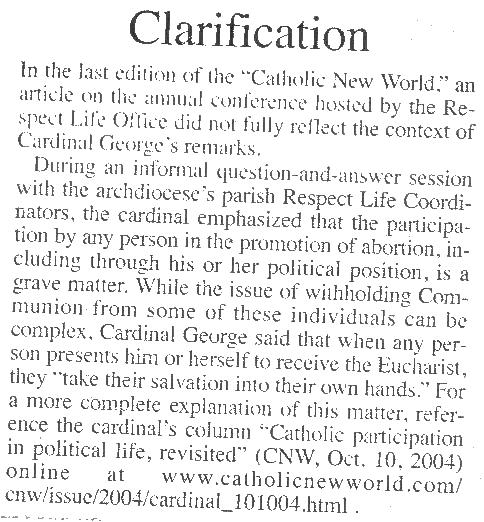
\includegraphics[width=\linewidth]{figures/original/12.jpg}
    \subcaption[]{}{}
    \label{fig:12_image_original}
  \end{subfigure}
  \begin{subfigure}[b]{0.33\textwidth}%
    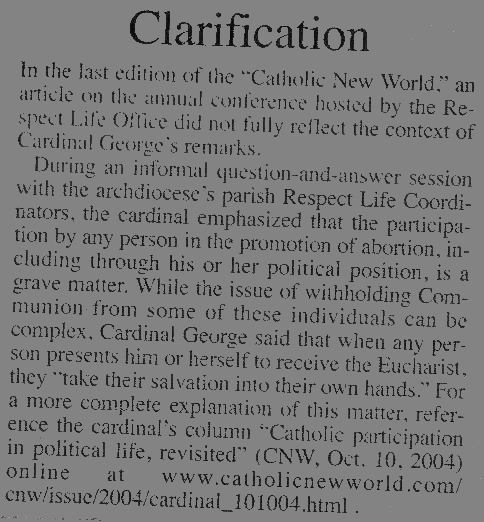
\includegraphics[width=\linewidth]{figures/hc_trap_split/12_output.jpg}
    \subcaption[]{}{}
    \label{fig:12_output_image_hc}
  \end{subfigure}
  \begin{subfigure}[b]{0.33\textwidth}%
    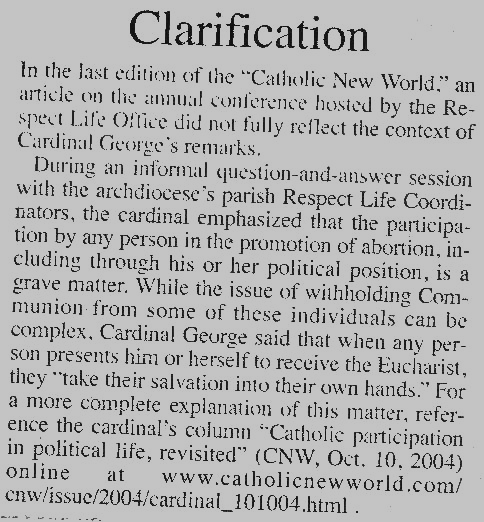
\includegraphics[width=\linewidth]{figures/ga_elitist/12_output.jpg}
    \subcaption[]{}{}
    \label{fig:12_output_image_ga}
  \end{subfigure}
  \caption{enhanced image generated by (b) simple HC (c) GA and (a) is original image}
  \label{fig:12_result}

  % one image
  \begin{subfigure}[b]{0.33\textwidth}
    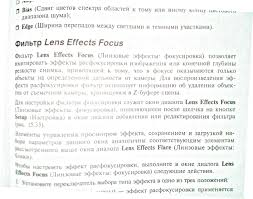
\includegraphics[width=\linewidth]{figures/original/13.jpg}
    \subcaption[]{}{}
    \label{fig:13_image_original}
  \end{subfigure}
  \begin{subfigure}[b]{0.33\textwidth}%
    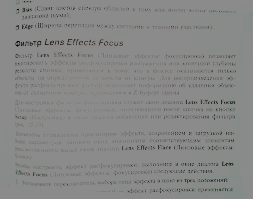
\includegraphics[width=\linewidth]{figures/hc_trap_split/13_output.jpg}
    \subcaption[]{}{}
    \label{fig:13_output_image_hc}
  \end{subfigure}
  \begin{subfigure}[b]{0.33\textwidth}%
    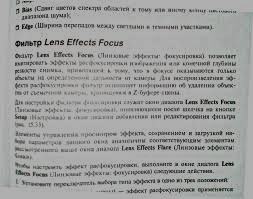
\includegraphics[width=\linewidth]{figures/ga_elitist/13_output.jpg}
    \subcaption[]{}{}
    \label{fig:13_output_image_ga}
  \end{subfigure}
  \caption{enhanced image generated by (b) simple HC (c) GA and (a) is original image}
  \label{fig:13_result}

  % one image
  \begin{subfigure}[b]{0.33\textwidth}
    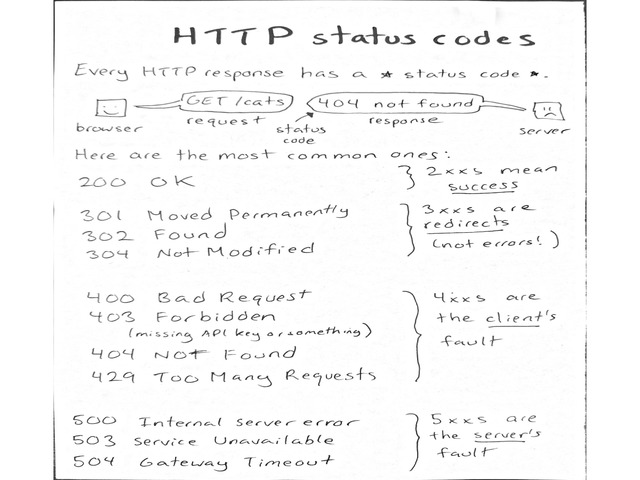
\includegraphics[width=\linewidth]{figures/original/09.jpg}
    \subcaption[]{}{}
    \label{fig:09_image_original}
  \end{subfigure}
  \begin{subfigure}[b]{0.33\textwidth}%
    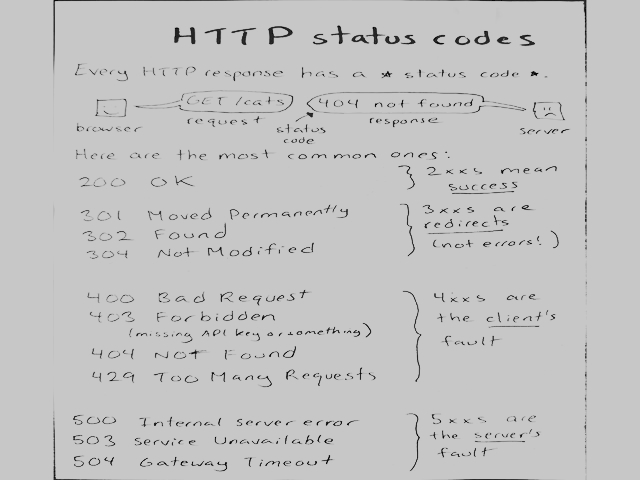
\includegraphics[width=\linewidth]{figures/hc_trap_split/09_output.jpg}
    \subcaption[]{}{}
    \label{fig:09_output_image_hc}
  \end{subfigure}
  \begin{subfigure}[b]{0.33\textwidth}%
    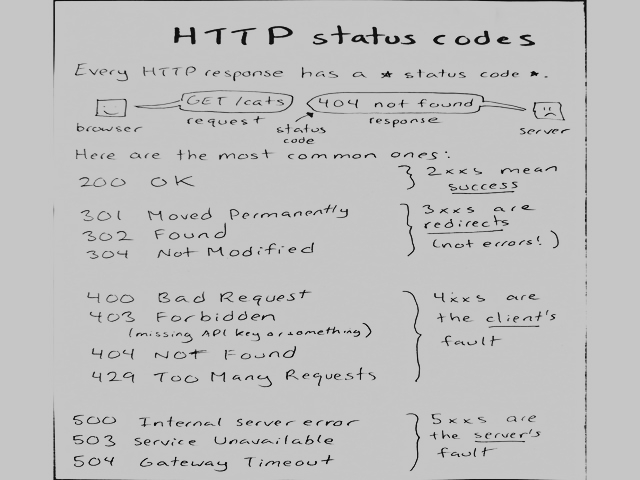
\includegraphics[width=\linewidth]{figures/ga_elitist/09_output.jpg}
    \subcaption[]{}{}
    \label{fig:09_output_image_ga}
  \end{subfigure}
  \caption{enhanced image generated by (b) simple HC (c) GA and (a) is original image}
  \label{fig:09_result}
\end{figure*}

% next page
\begin{figure*}
  % one image
  \begin{subfigure}[b]{0.33\textwidth}
    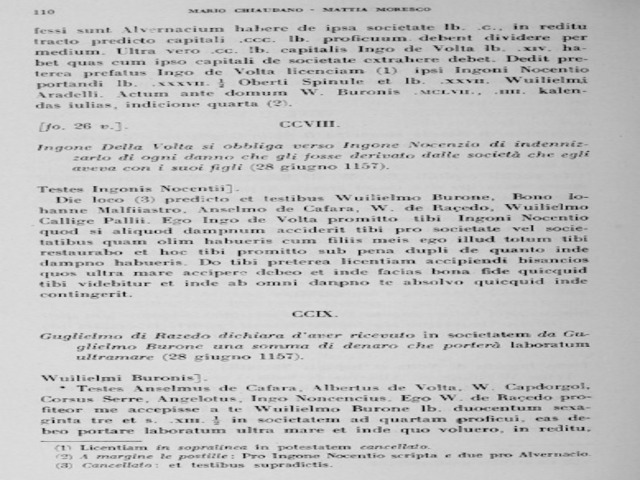
\includegraphics[width=\linewidth]{figures/original/10.jpg}
    \subcaption[]{}{}
    \label{fig:10_image_original}
  \end{subfigure}
  \begin{subfigure}[b]{0.33\textwidth}%
    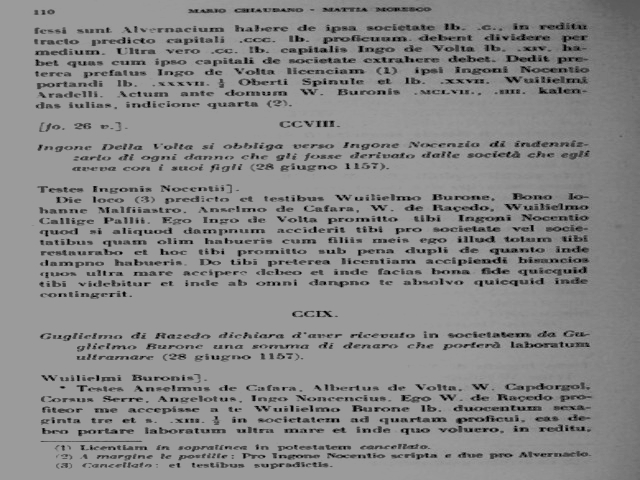
\includegraphics[width=\linewidth]{figures/hc_trap_split/10_output.jpg}
    \subcaption[]{}{}
    \label{fig:10_output_image_hc}
  \end{subfigure}
  \begin{subfigure}[b]{0.33\textwidth}%
    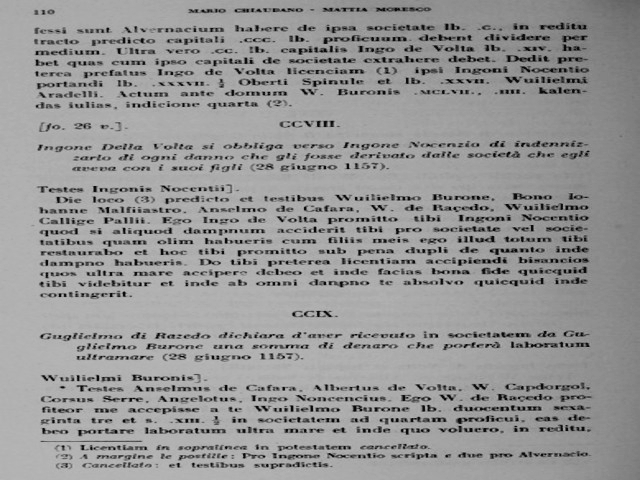
\includegraphics[width=\linewidth]{figures/ga_elitist/10_output.jpg}
    \subcaption[]{}{}
    \label{fig:10_output_image_ga}
  \end{subfigure}
  \caption{enhanced image generated by (b) simple HC (c) GA and (a) is original image}
  \label{fig:10_result}

  % one image
  \begin{subfigure}[b]{0.33\textwidth}
    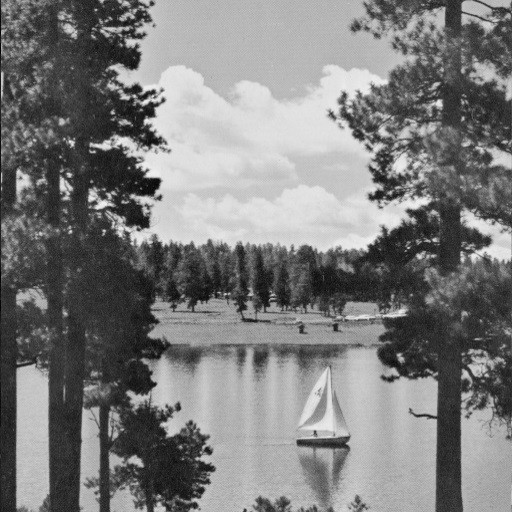
\includegraphics[width=\linewidth]{figures/original/lake.jpg}
    \subcaption[]{}{}
    \label{fig:lake_image_original}
  \end{subfigure}
  \begin{subfigure}[b]{0.33\textwidth}%
    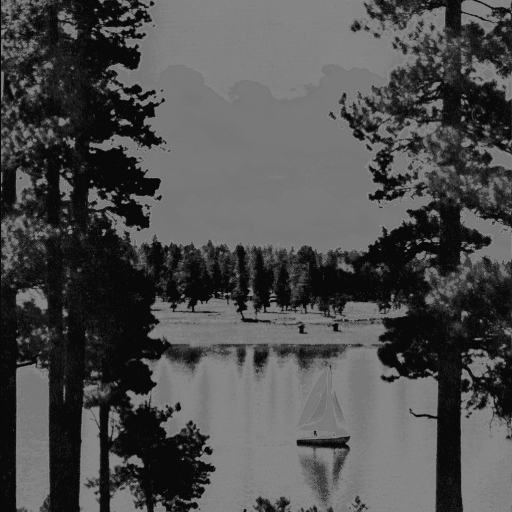
\includegraphics[width=\linewidth]{figures/hc_trap_split/lake_output.jpg}
    \subcaption[]{}{}
    \label{fig:lake_output_image_hc}
  \end{subfigure}
  \begin{subfigure}[b]{0.33\textwidth}%
    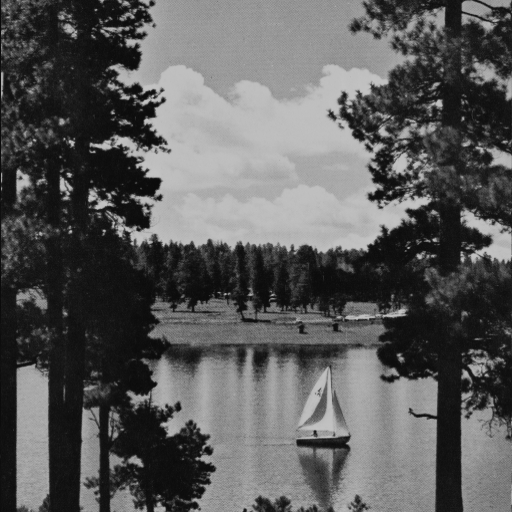
\includegraphics[width=\linewidth]{figures/ga_elitist/lake_output.jpg}
    \subcaption[]{}{}
    \label{fig:lake_output_image_ga}
  \end{subfigure}
  \caption{enhanced image generated by (b) simple HC (c) GA and (a) is original image}
  \label{fig:lake_result}

  % one image
  \begin{subfigure}[b]{0.33\textwidth}
    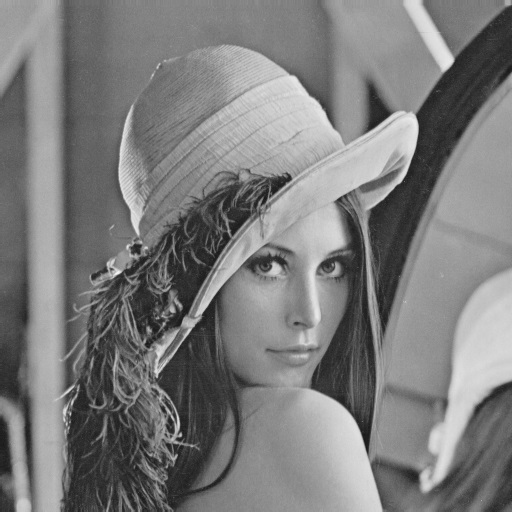
\includegraphics[width=\linewidth]{figures/original/lena_gray_512.jpg}
    \subcaption[]{}{}
    \label{fig:lenagray_image_original}
  \end{subfigure}
  \begin{subfigure}[b]{0.33\textwidth}%
    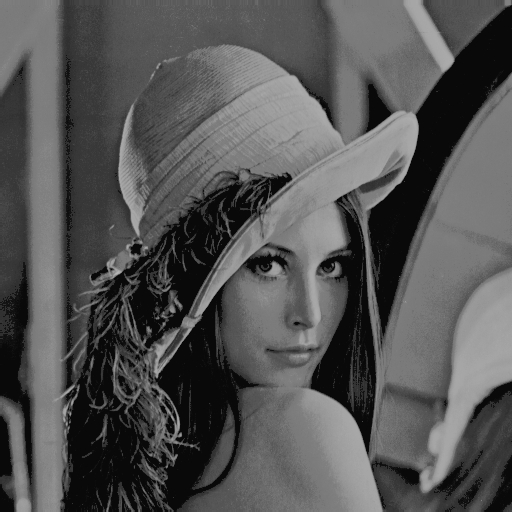
\includegraphics[width=\linewidth]{figures/hc_trap_split/lena_gray_512_output.jpg}
    \subcaption[]{}{}
    \label{fig:lenagray_output_image_hc}
  \end{subfigure}
  \begin{subfigure}[b]{0.33\textwidth}%
    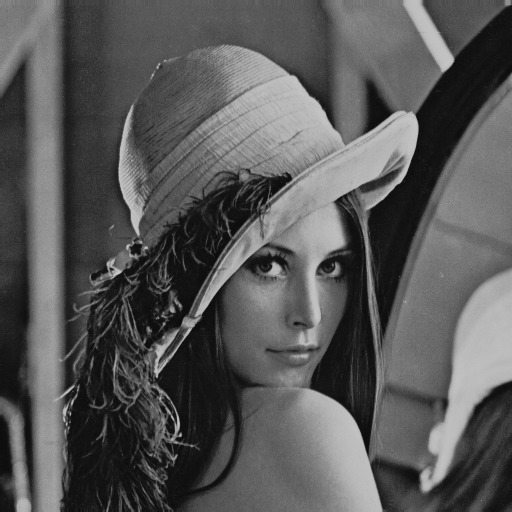
\includegraphics[width=\linewidth]{figures/ga_elitist/lena_gray_512_output.jpg}
    \subcaption[]{}{}
    \label{fig:lenagray_output_image_ga}
  \end{subfigure}
  \caption{enhanced image generated by (b) simple HC (c) GA and (a) is original image}
  \label{fig:lenagray_result}
\end{figure*}

% next page
\begin{figure*}
  % one image
  \begin{subfigure}[b]{0.33\textwidth}
    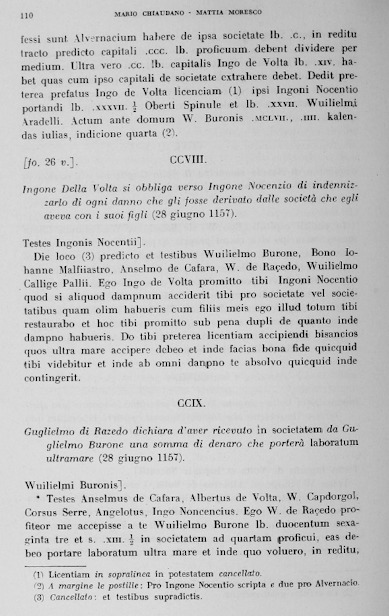
\includegraphics[width=\linewidth]{figures/original/06.jpg}
    \subcaption[]{}{}
    \label{fig:06_image_original}
  \end{subfigure}
  \begin{subfigure}[b]{0.33\textwidth}%
    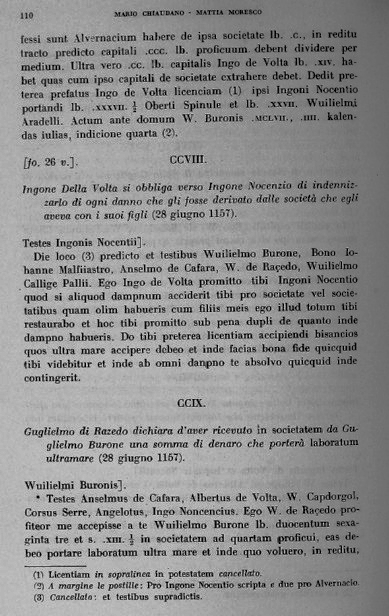
\includegraphics[width=\linewidth]{figures/hc_trap_split/06_output.jpg}
    \subcaption[]{}{}
    \label{fig:06_output_image_hc}
  \end{subfigure}
  \begin{subfigure}[b]{0.33\textwidth}%
    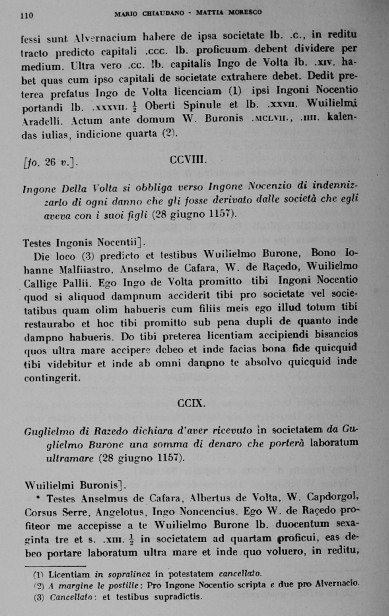
\includegraphics[width=\linewidth]{figures/ga_elitist/06_output.jpg}
    \subcaption[]{}{}
    \label{fig:06_output_image_ga}
  \end{subfigure}
  \caption{enhanced image generated by (b) simple HC (c) GA and (a) is original image}
  \label{fig:06_result}

  % one image
  \begin{subfigure}[b]{0.33\textwidth}
    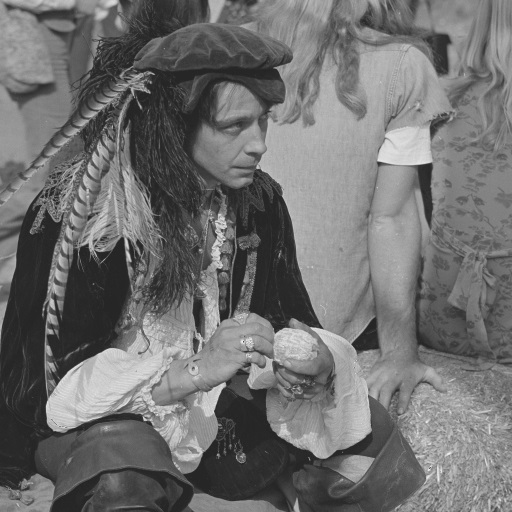
\includegraphics[width=\linewidth]{figures/original/pirate.jpg}
    \subcaption[]{}{}
    \label{fig:pirate_image_original}
  \end{subfigure}
  \begin{subfigure}[b]{0.33\textwidth}%
    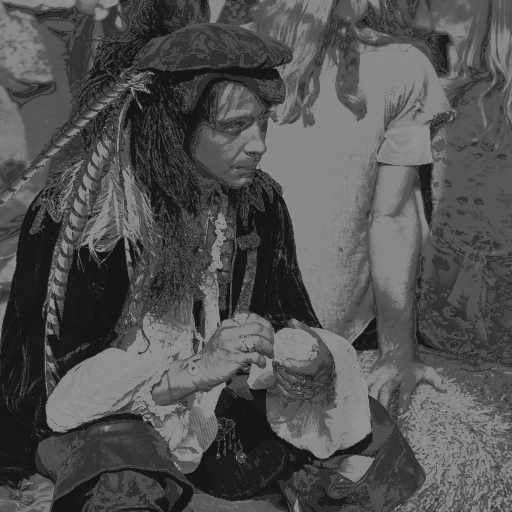
\includegraphics[width=\linewidth]{figures/hc_trap_split/pirate_output.jpg}
    \subcaption[]{}{}
    \label{fig:pirate_output_image_hc}
  \end{subfigure}
  \begin{subfigure}[b]{0.33\textwidth}%
    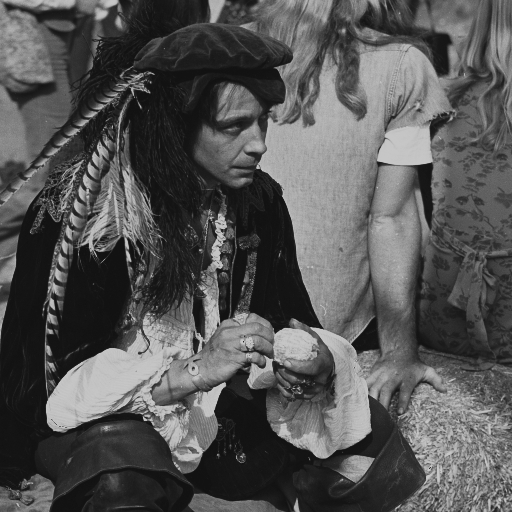
\includegraphics[width=\linewidth]{figures/ga_elitist/pirate_output.jpg}
    \subcaption[]{}{}
    \label{fig:pirate_output_image_ga}
  \end{subfigure}
  \caption{enhanced image generated by (b) simple HC (c) GA and (a) is original image}
  \label{fig:pirate_result}
\end{figure*}